\chapter{Working} 
\begin{itemize}
	\item 9V Battery is connected to the helmet section. After successful connection LED on the helmet unit will turn on.
	\item Power adapter is used to power up the bike section. Whereas in case of its connection with bike it will be connected to the ignition switch in the bike which look like as image shown below.
	\begin{figure}[h]
		\centering
		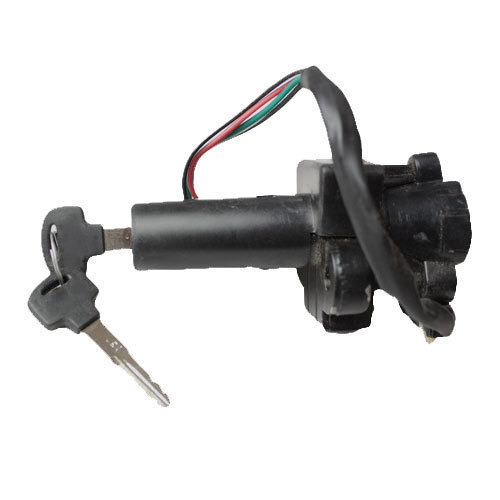
\includegraphics[scale=.25]{ignition-switch-lock-1-500x500.jpg}
		\caption{Ignition Switch.}
	\end{figure}
	\item Red colour led glowing on Alchohol sensor(MQ3) indicates that the sensor is active.
	\item If the helmet is buckled up and the Limt Switch is on then the RF Transmitter will start communicating with the RF Reciever. \item The signal is encoded by HT12E encoder in the helmet unit and decoded by HT12D decoder in the RF Receiver circuit.
	
	\begin{figure}[h]
		\centering
		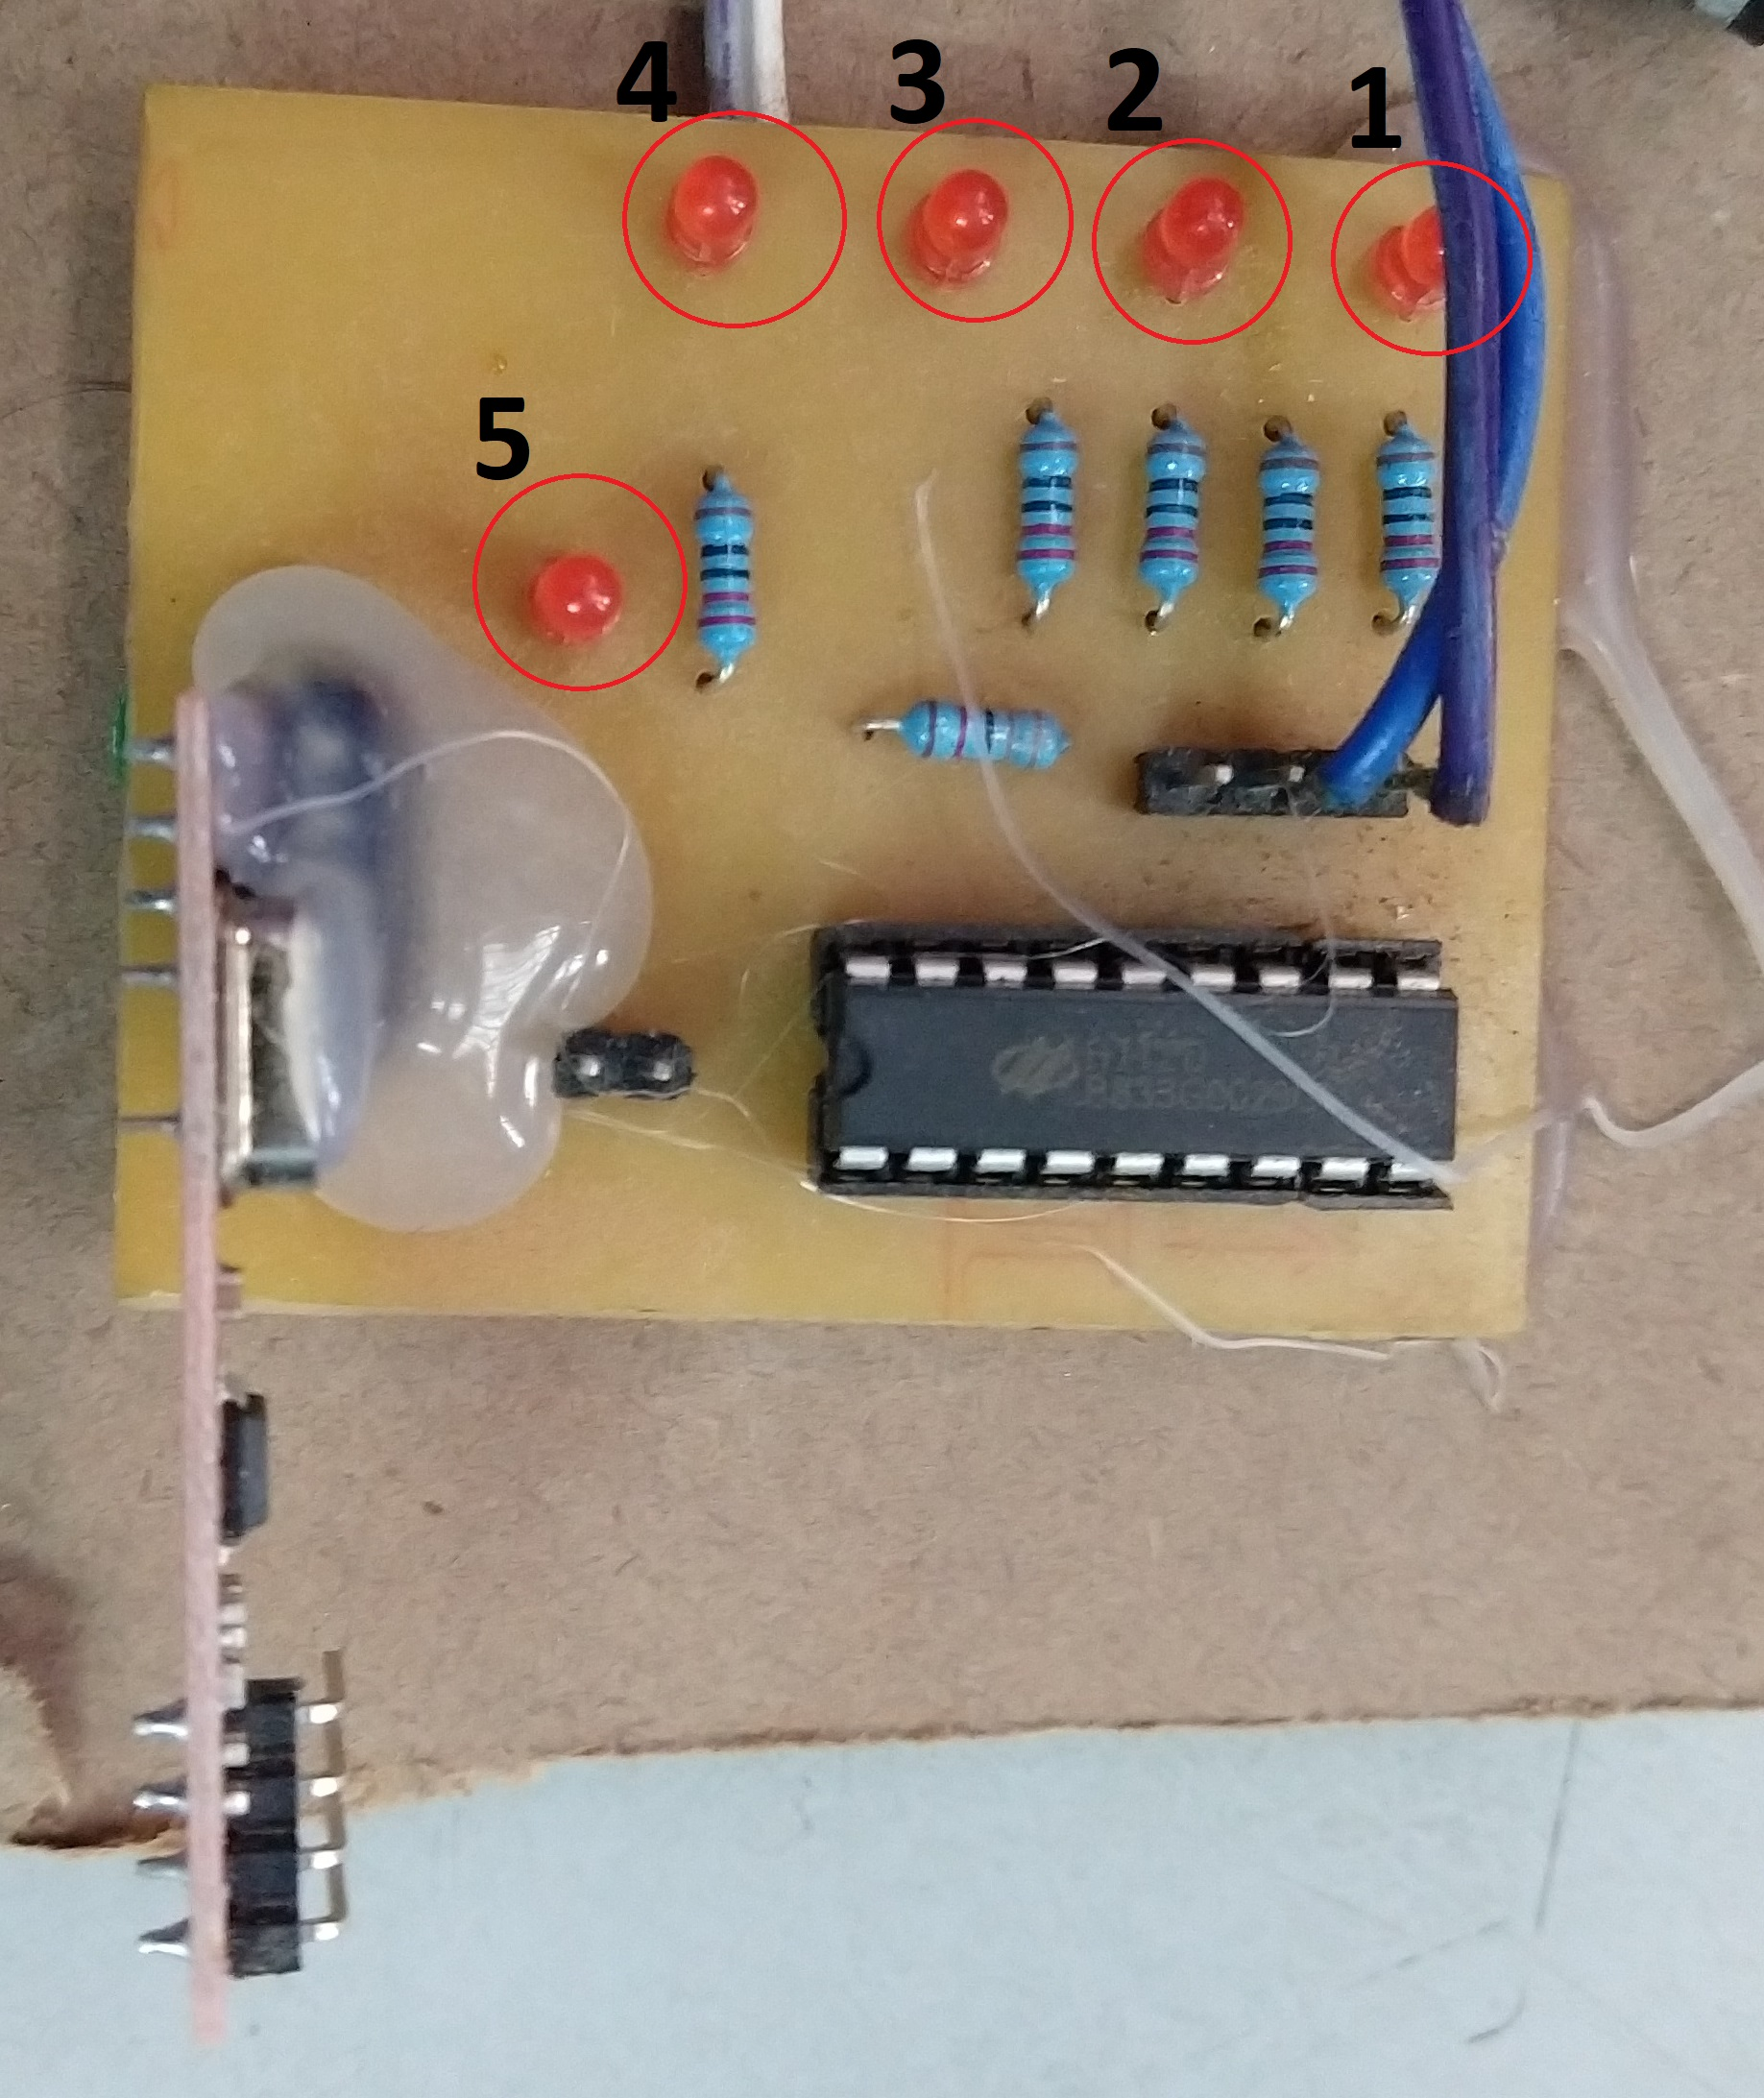
\includegraphics[scale=.09]{IMG_20210617_140308604 - Copy.jpg}
		\caption{RF Receiver Section.}
	\end{figure}
	\item In RF Receiver section 5th LED will turn on after recieving power (either by bike or power supply) whenever the helmet unit is in range of communication with bike unit.
	\item 1st LED will turn on or off if the limit switch is pressed or not.
	\item 2nd LED will turn on and off as per the signal from alchohol sensor.
	\item 3rd LED will turn on and off as per the 12V DC Motor relay circuit.
	\item 4th Led will turn on as per the GSM Module.
	\item Received signal is transferred to ATmega328 for processing.
	\begin{figure}[h]
		\centering
		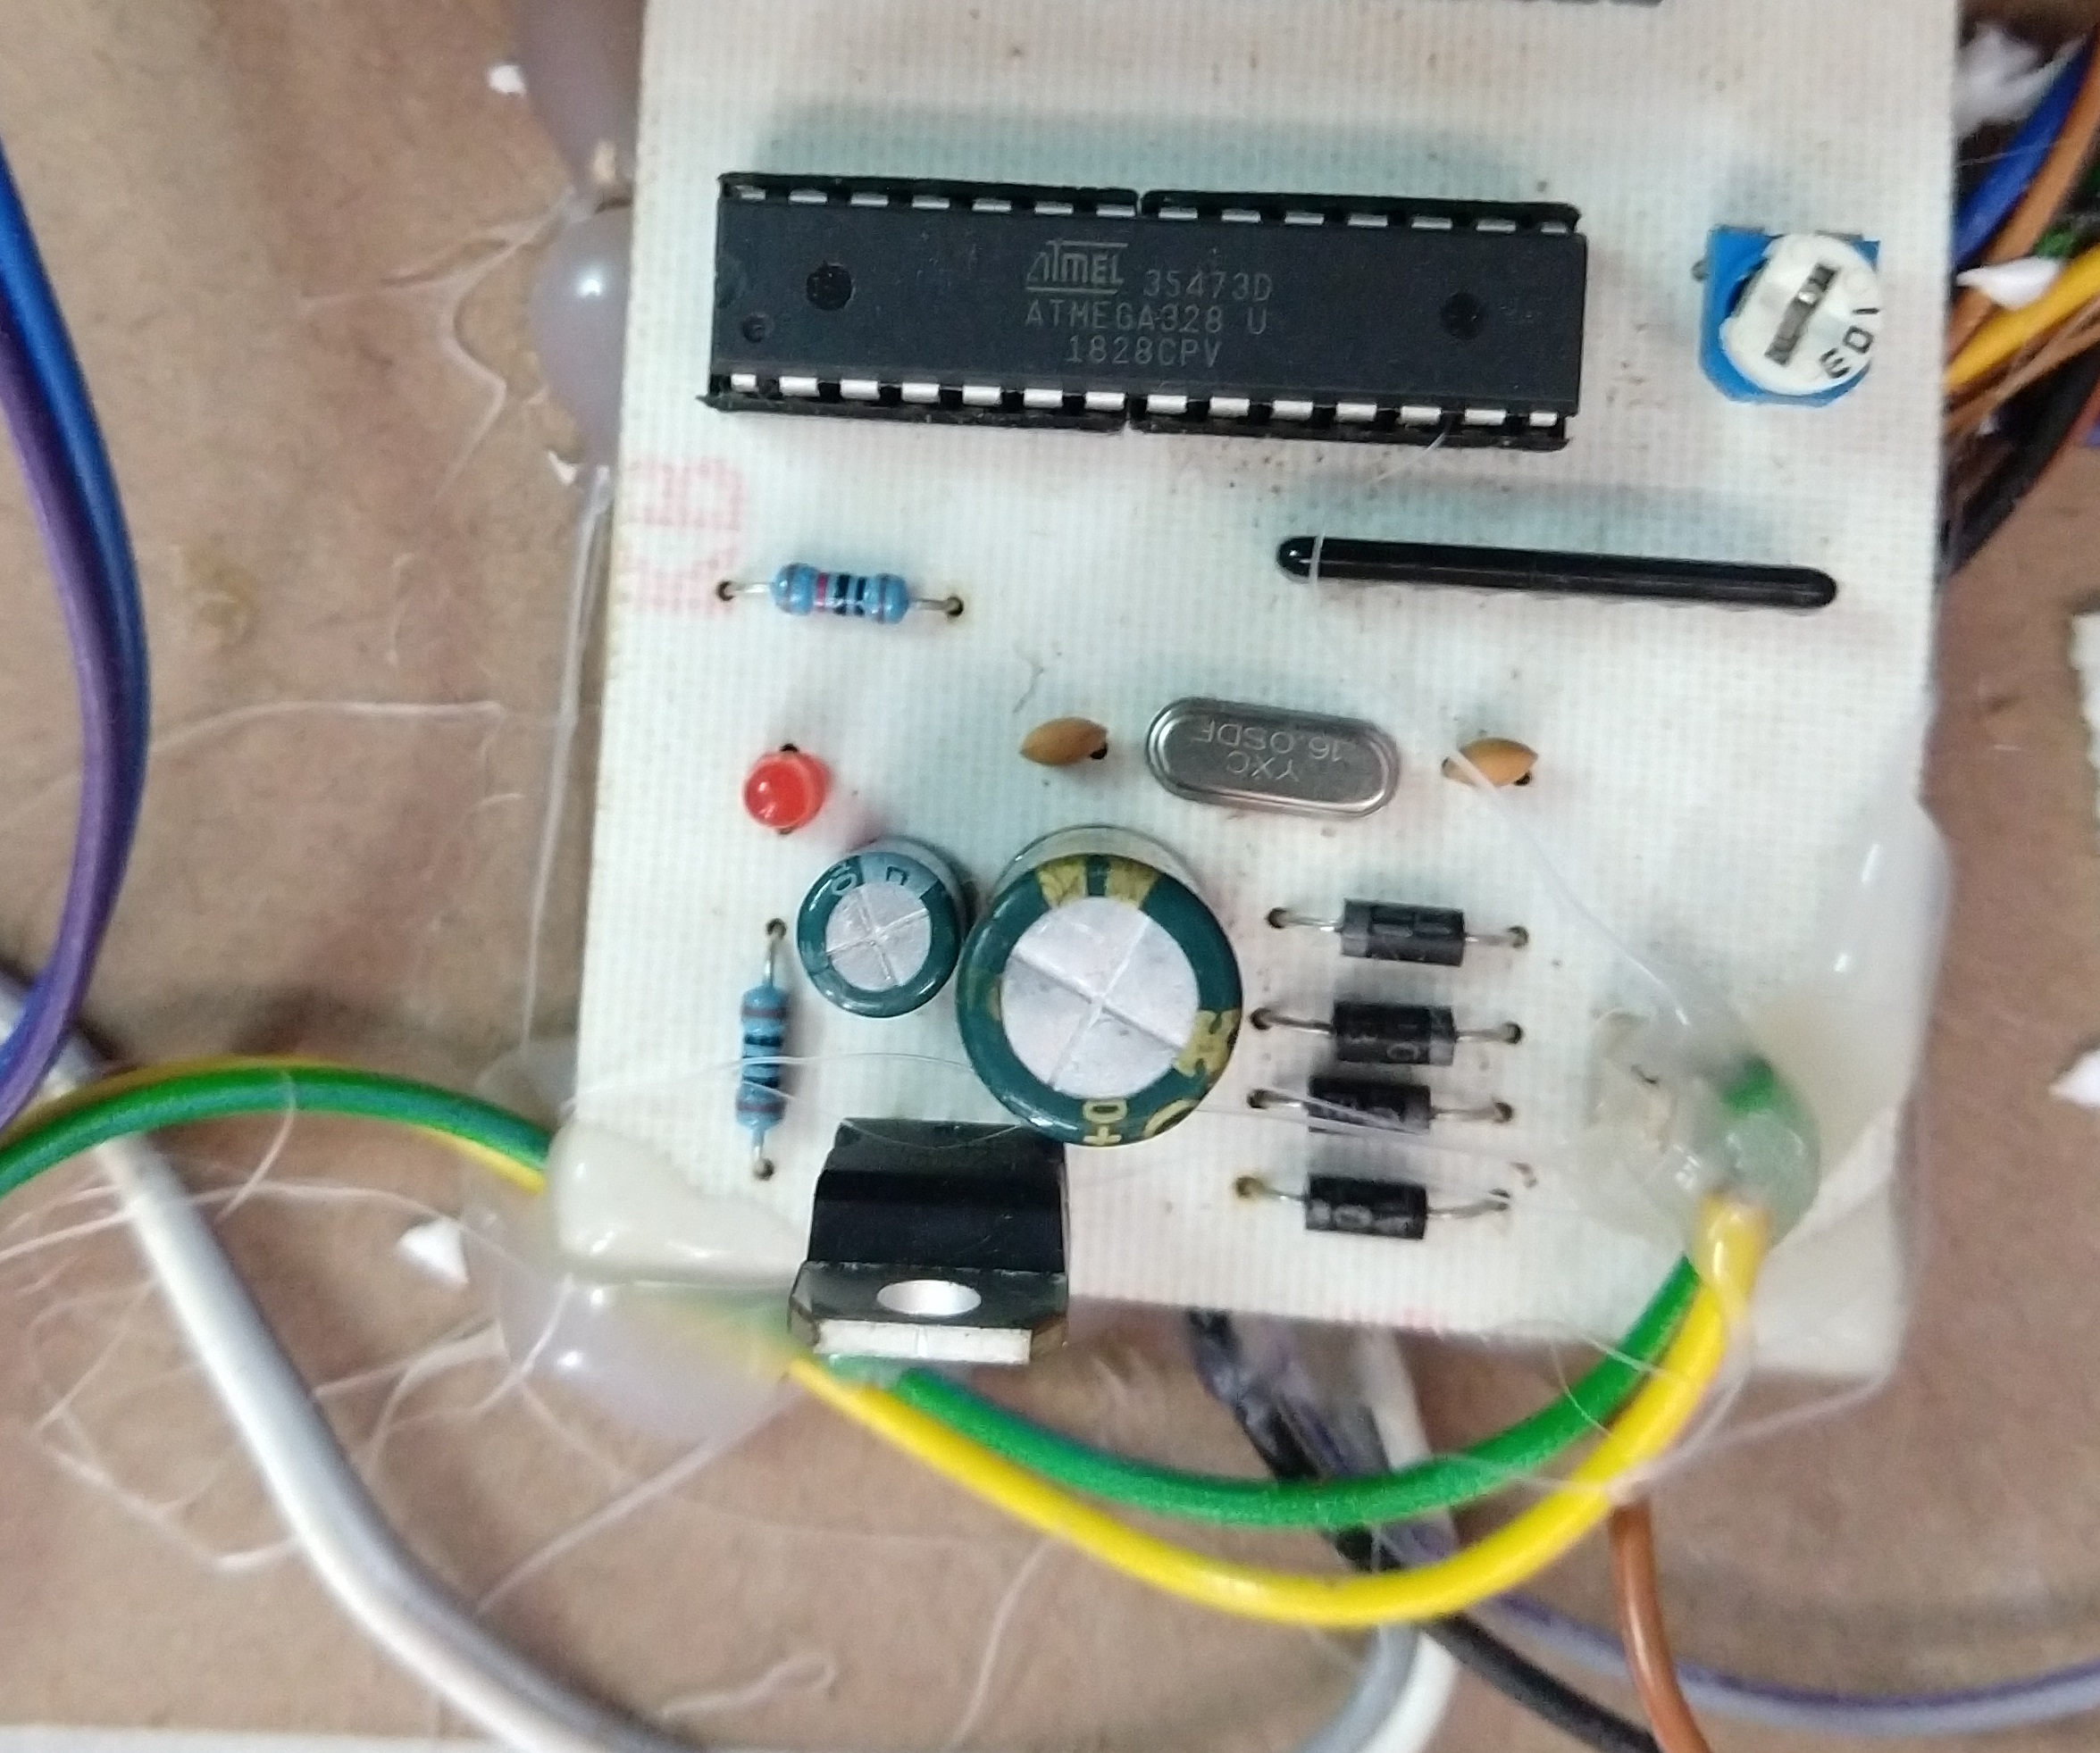
\includegraphics[scale=.1]{IMG_20210617_140313983.jpg}
		\caption{Heart Of System.}
	\end{figure}
	
	\item Atmega 328 IC is the heart and brain of this system. It manages all the other devices.
	\begin{figure}[h]
		\centering
		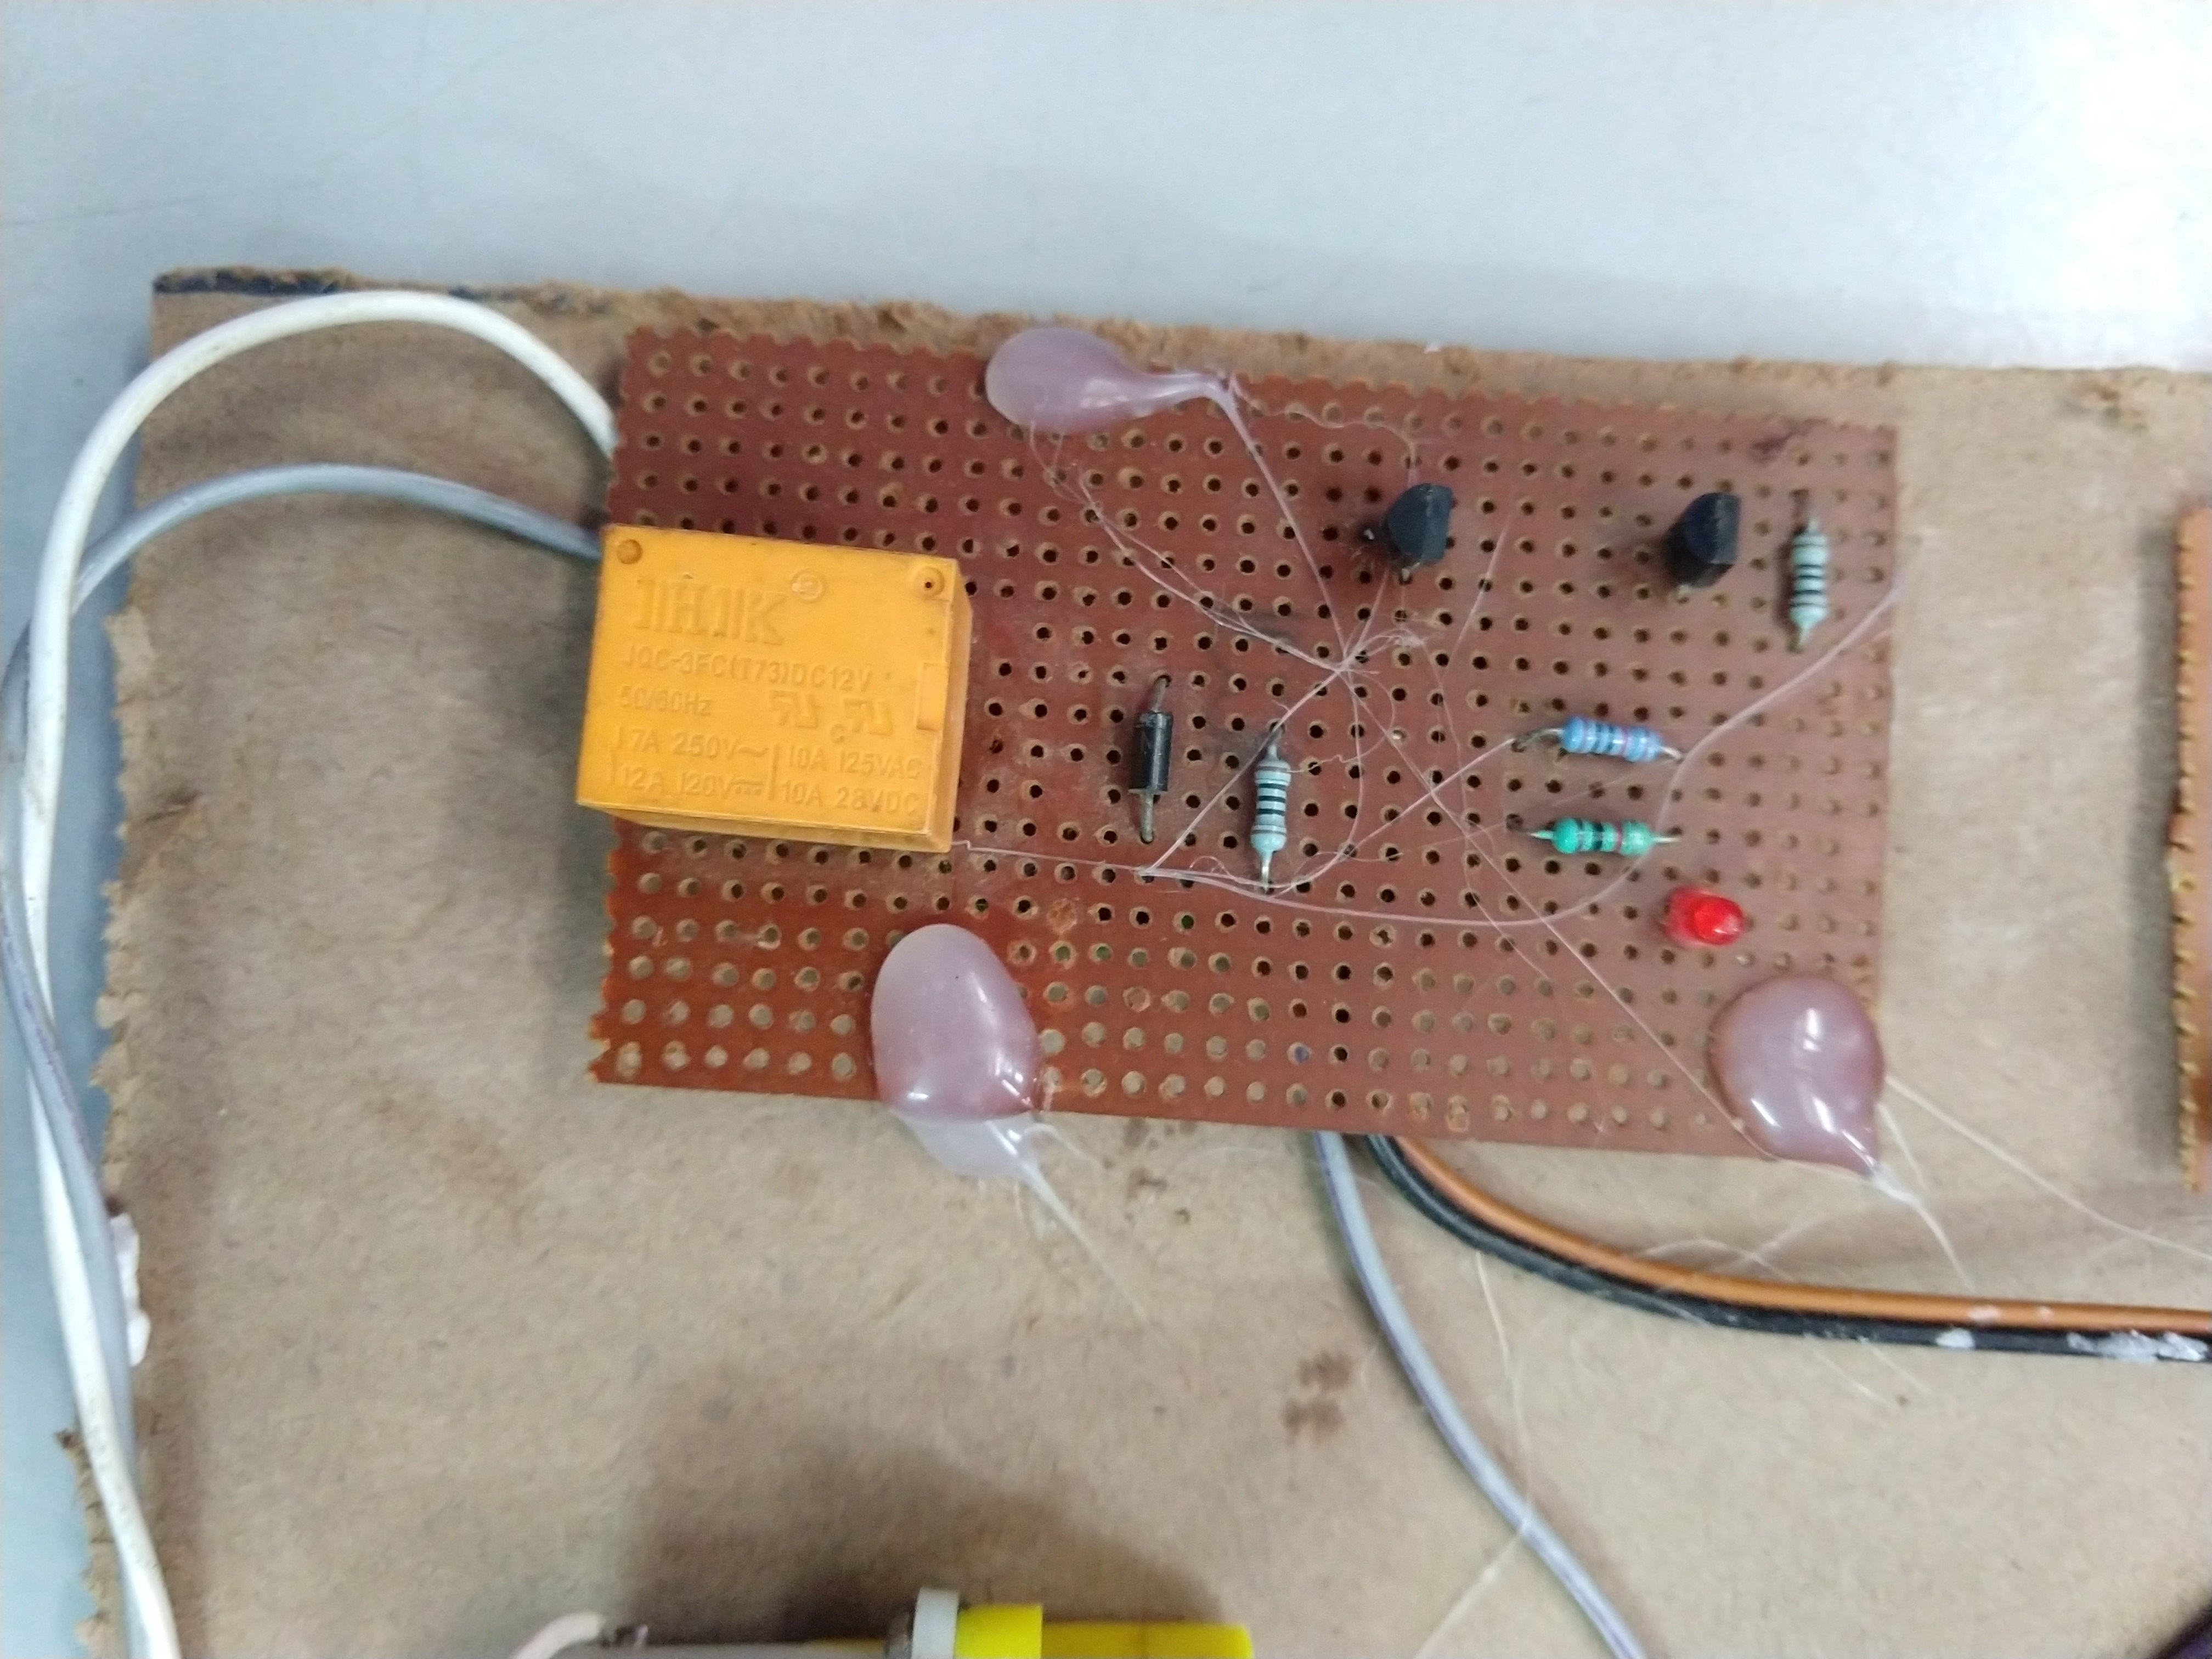
\includegraphics[scale=.035]{IMG_20210617_140318107.jpg}
		\caption{Relay Circuit.}
	\end{figure}
	\begin{itemize}
		\item It manages relay circuit as per the signal received from helmet unit, and relay manages the 12V motor.
		
		
		\begin{figure}[h]
			\centering
			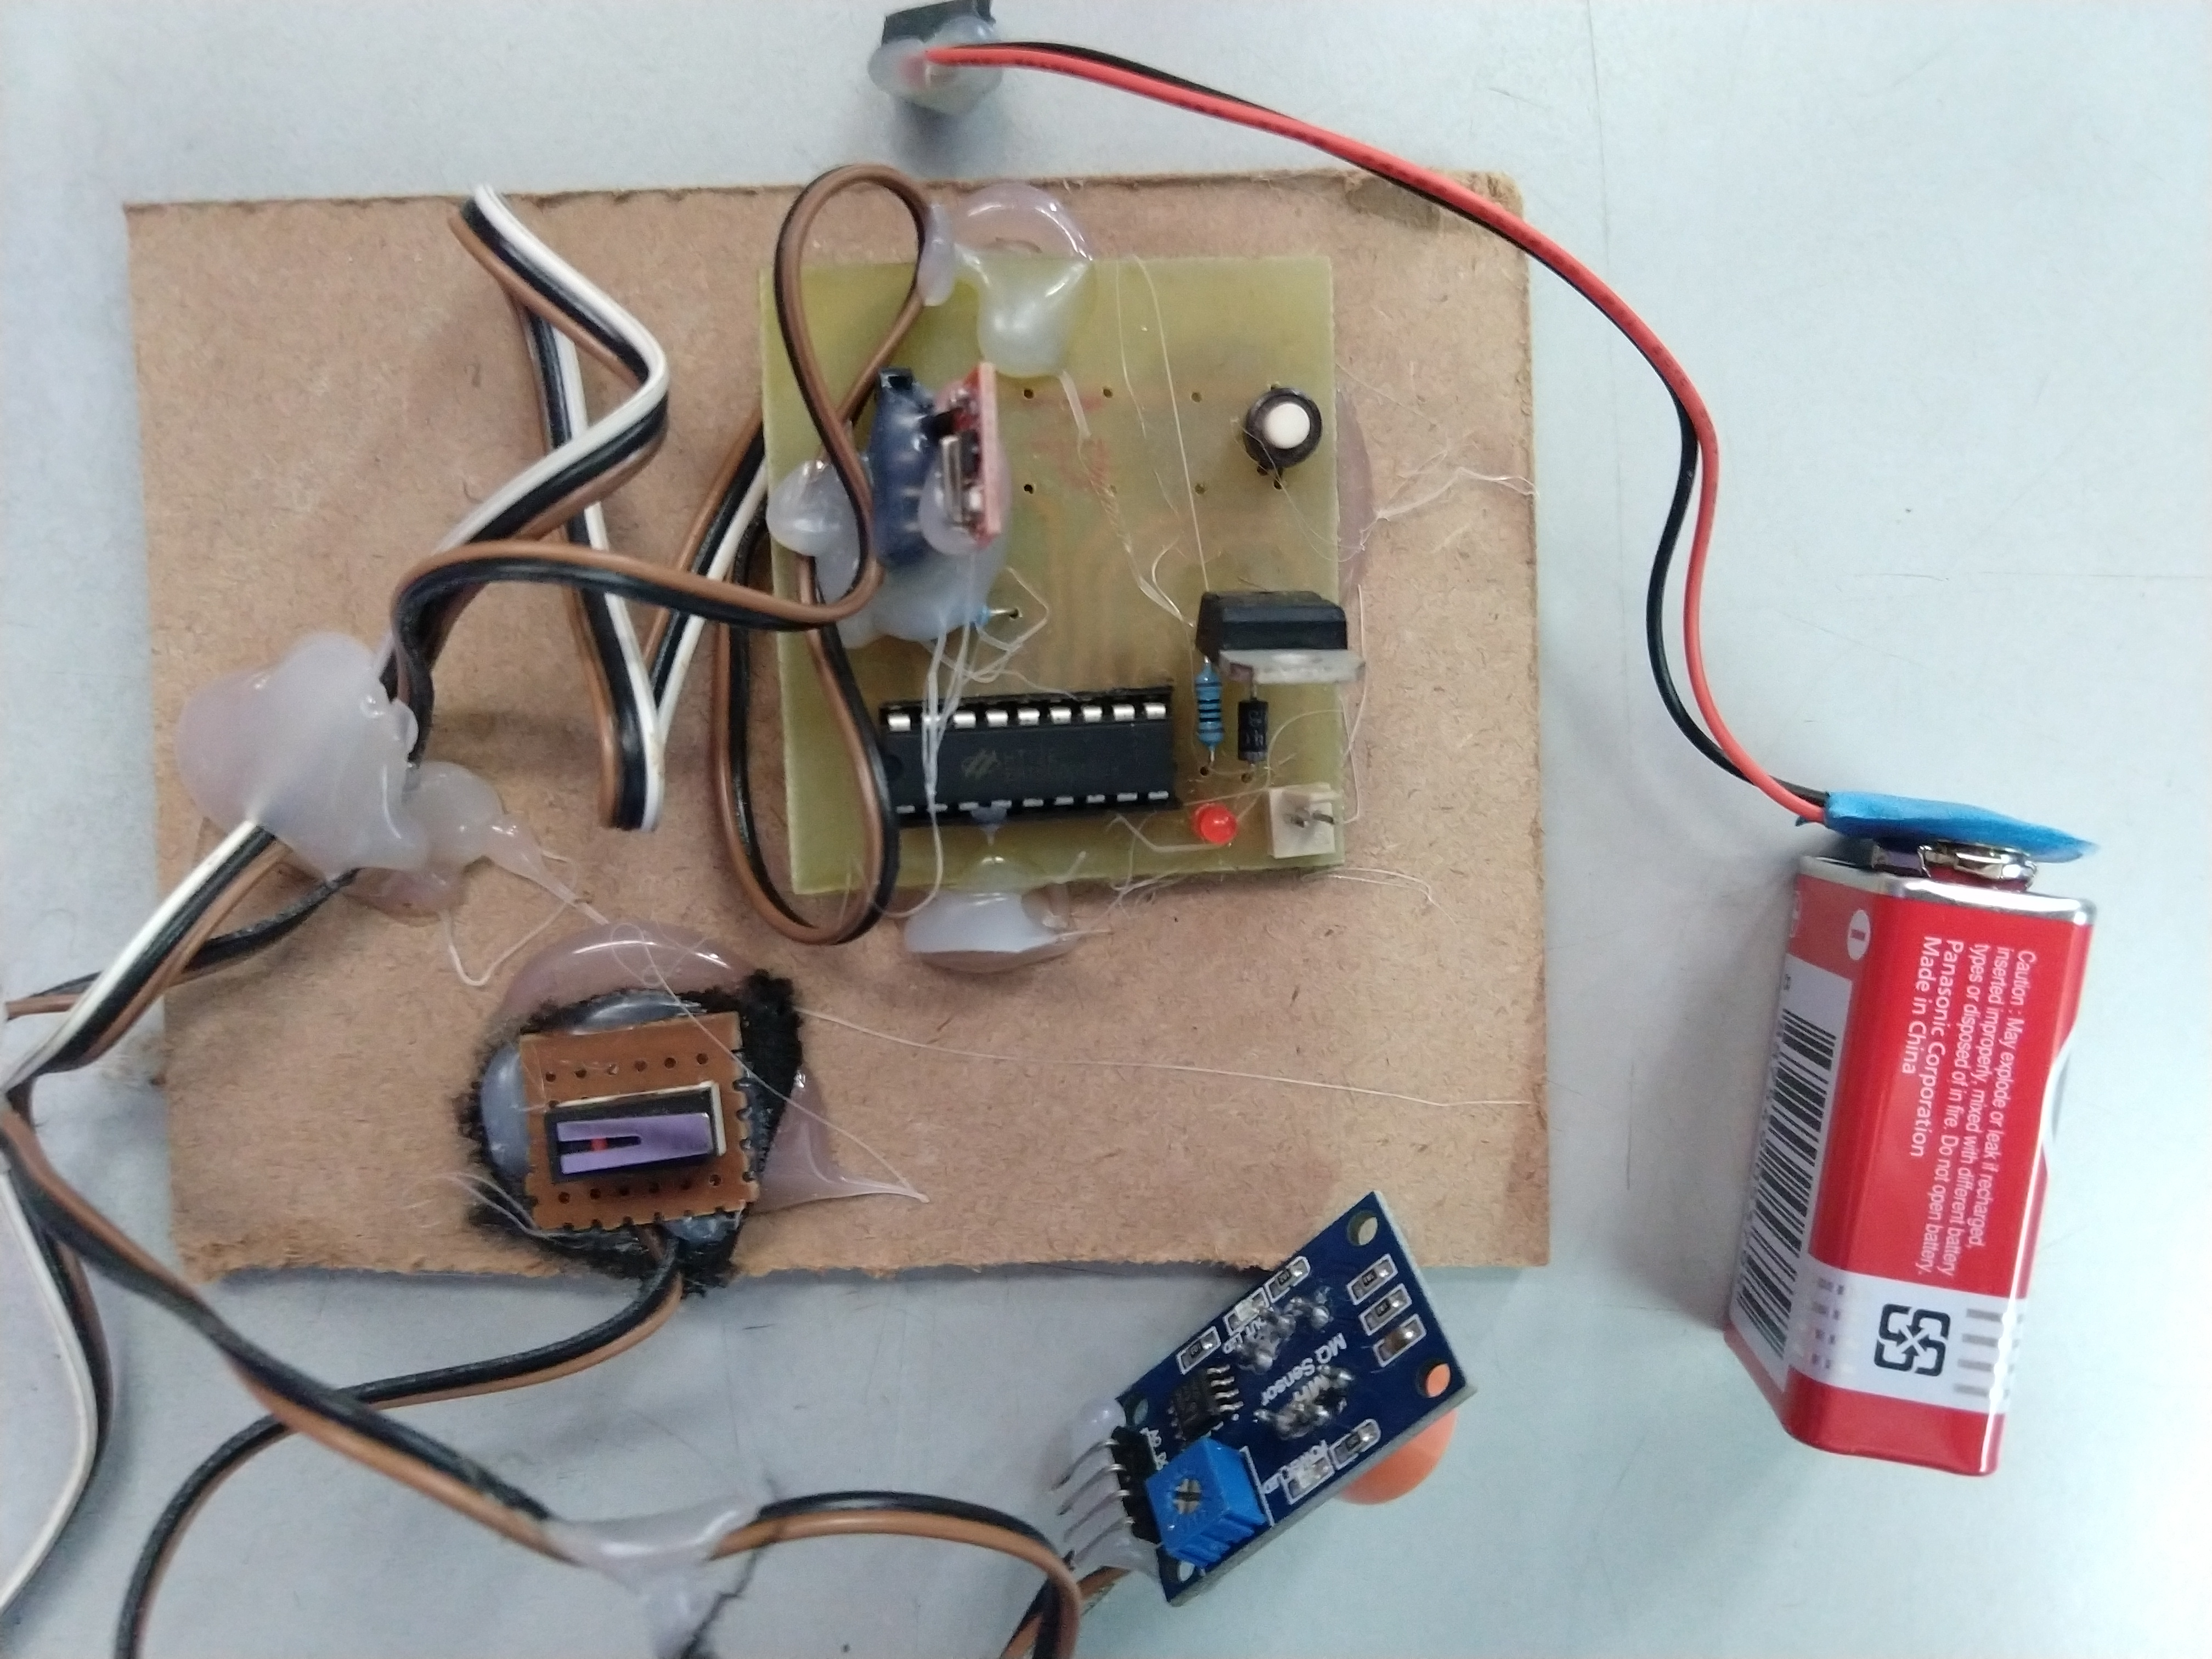
\includegraphics[scale=.04]{IMG_20210617_140708629.jpg}
			\caption{Helmet Unit.}
		\end{figure}
		\item GSM Module is triggerred by the action of reed switches	 
	\end{itemize}
	
	\item Current status of system will appear on LCD display.
	
\end{itemize}

\section{Working Conditions}
\subsection{Pressence Of Alchohol}
\begin{itemize}
	\item When MQ3 sensor detects alchohol then a green LED in the MQ3 sensor glows up and it sends a signal to the HT12E encoder.
	\begin{figure}[h]
		\centering
		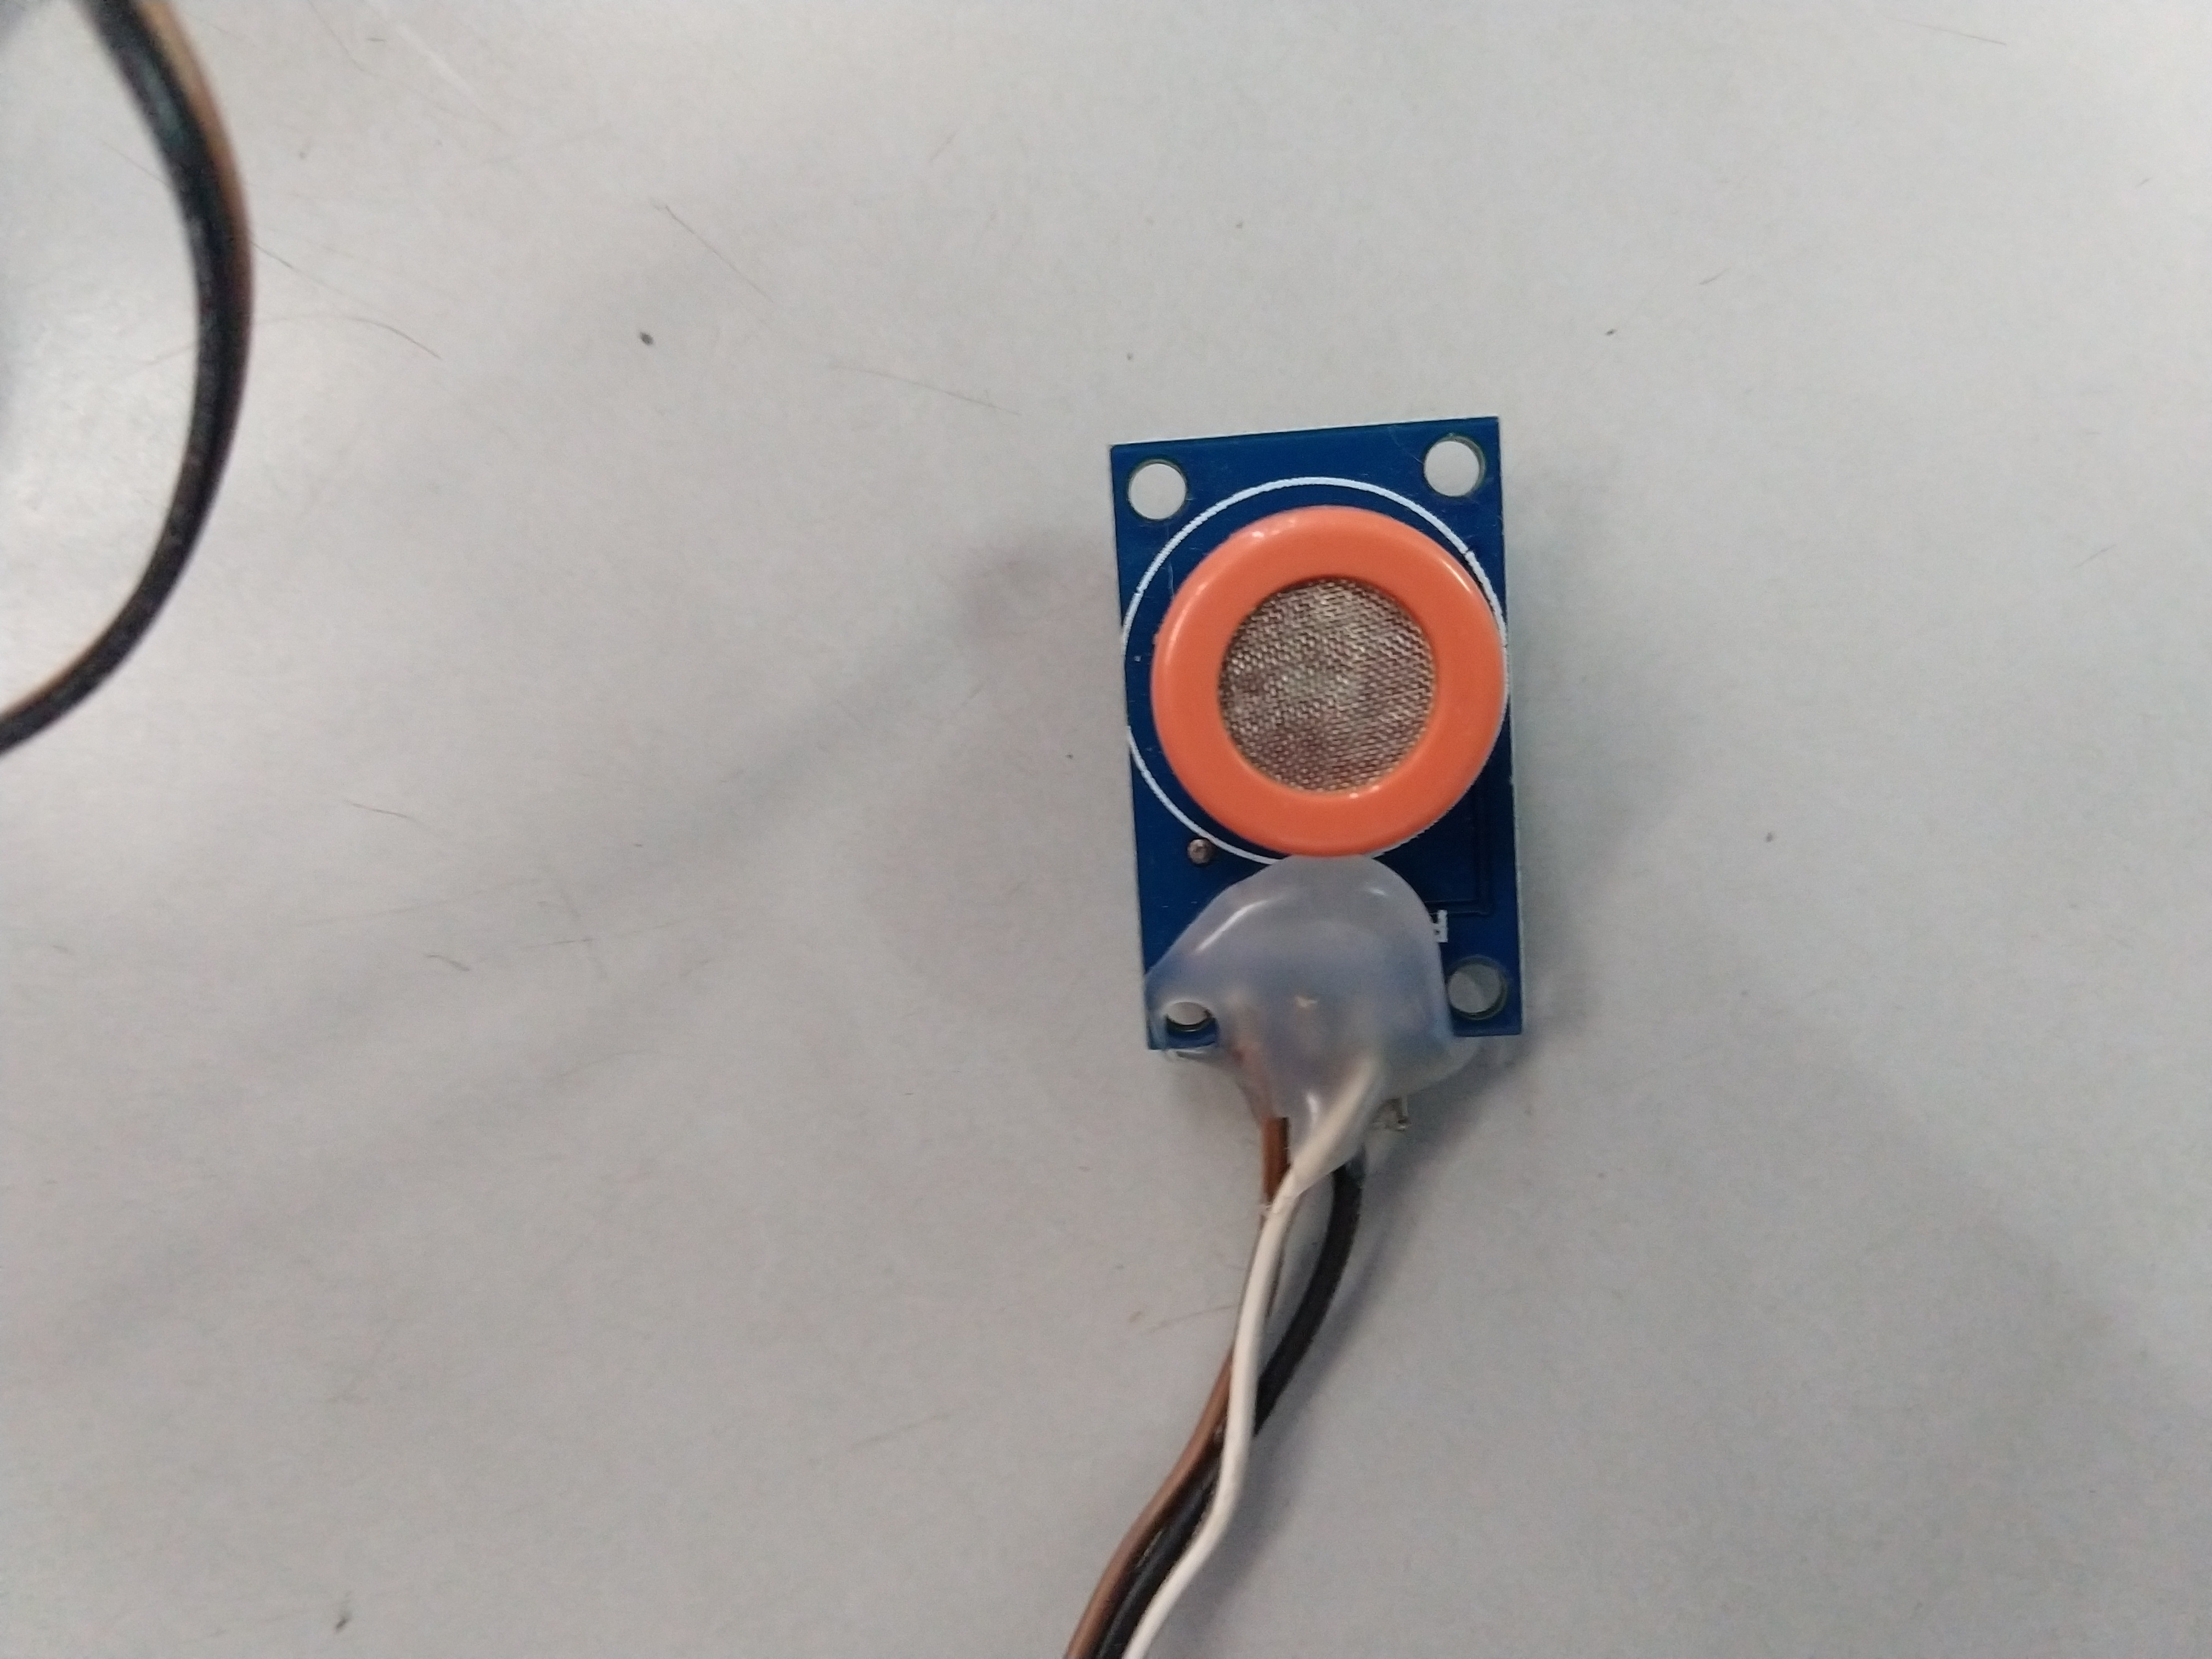
\includegraphics[scale=.05]{IMG_20210617_140538144.jpg}
		\caption{MQ3 Sensor.}
	\end{figure} 
	\item HT12E sends the encoded signal to RF transmitter.
	\item Then at bike end RF receiver recieves signal and send it to HT12D decoder.
	\item The decoded message is then fed to ATmega328 which acts on the message.
	\item ATmega328 sends a signal to relay circuit to stop the ignition and send on message to the buzzer unit.
	\begin{figure}[h]
		\centering
		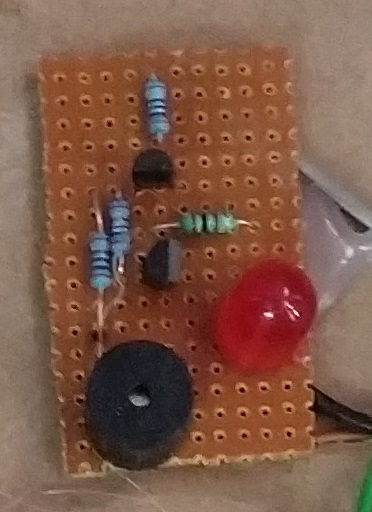
\includegraphics[scale=.5]{IMG_20210617_140301651 - Copy.jpg}
		\caption{Buzzer Circuit.}
	\end{figure}
	\item LCD display will show message that "ALCOHOL DETECTED".
\end{itemize}

\pagebreak
\subsection{Rider Wearing Helmet Or Not?}
\begin{itemize}
	\item We are using limit switches to detect the pressence of helmet on rider.
	\begin{figure}[h]
		\centering
		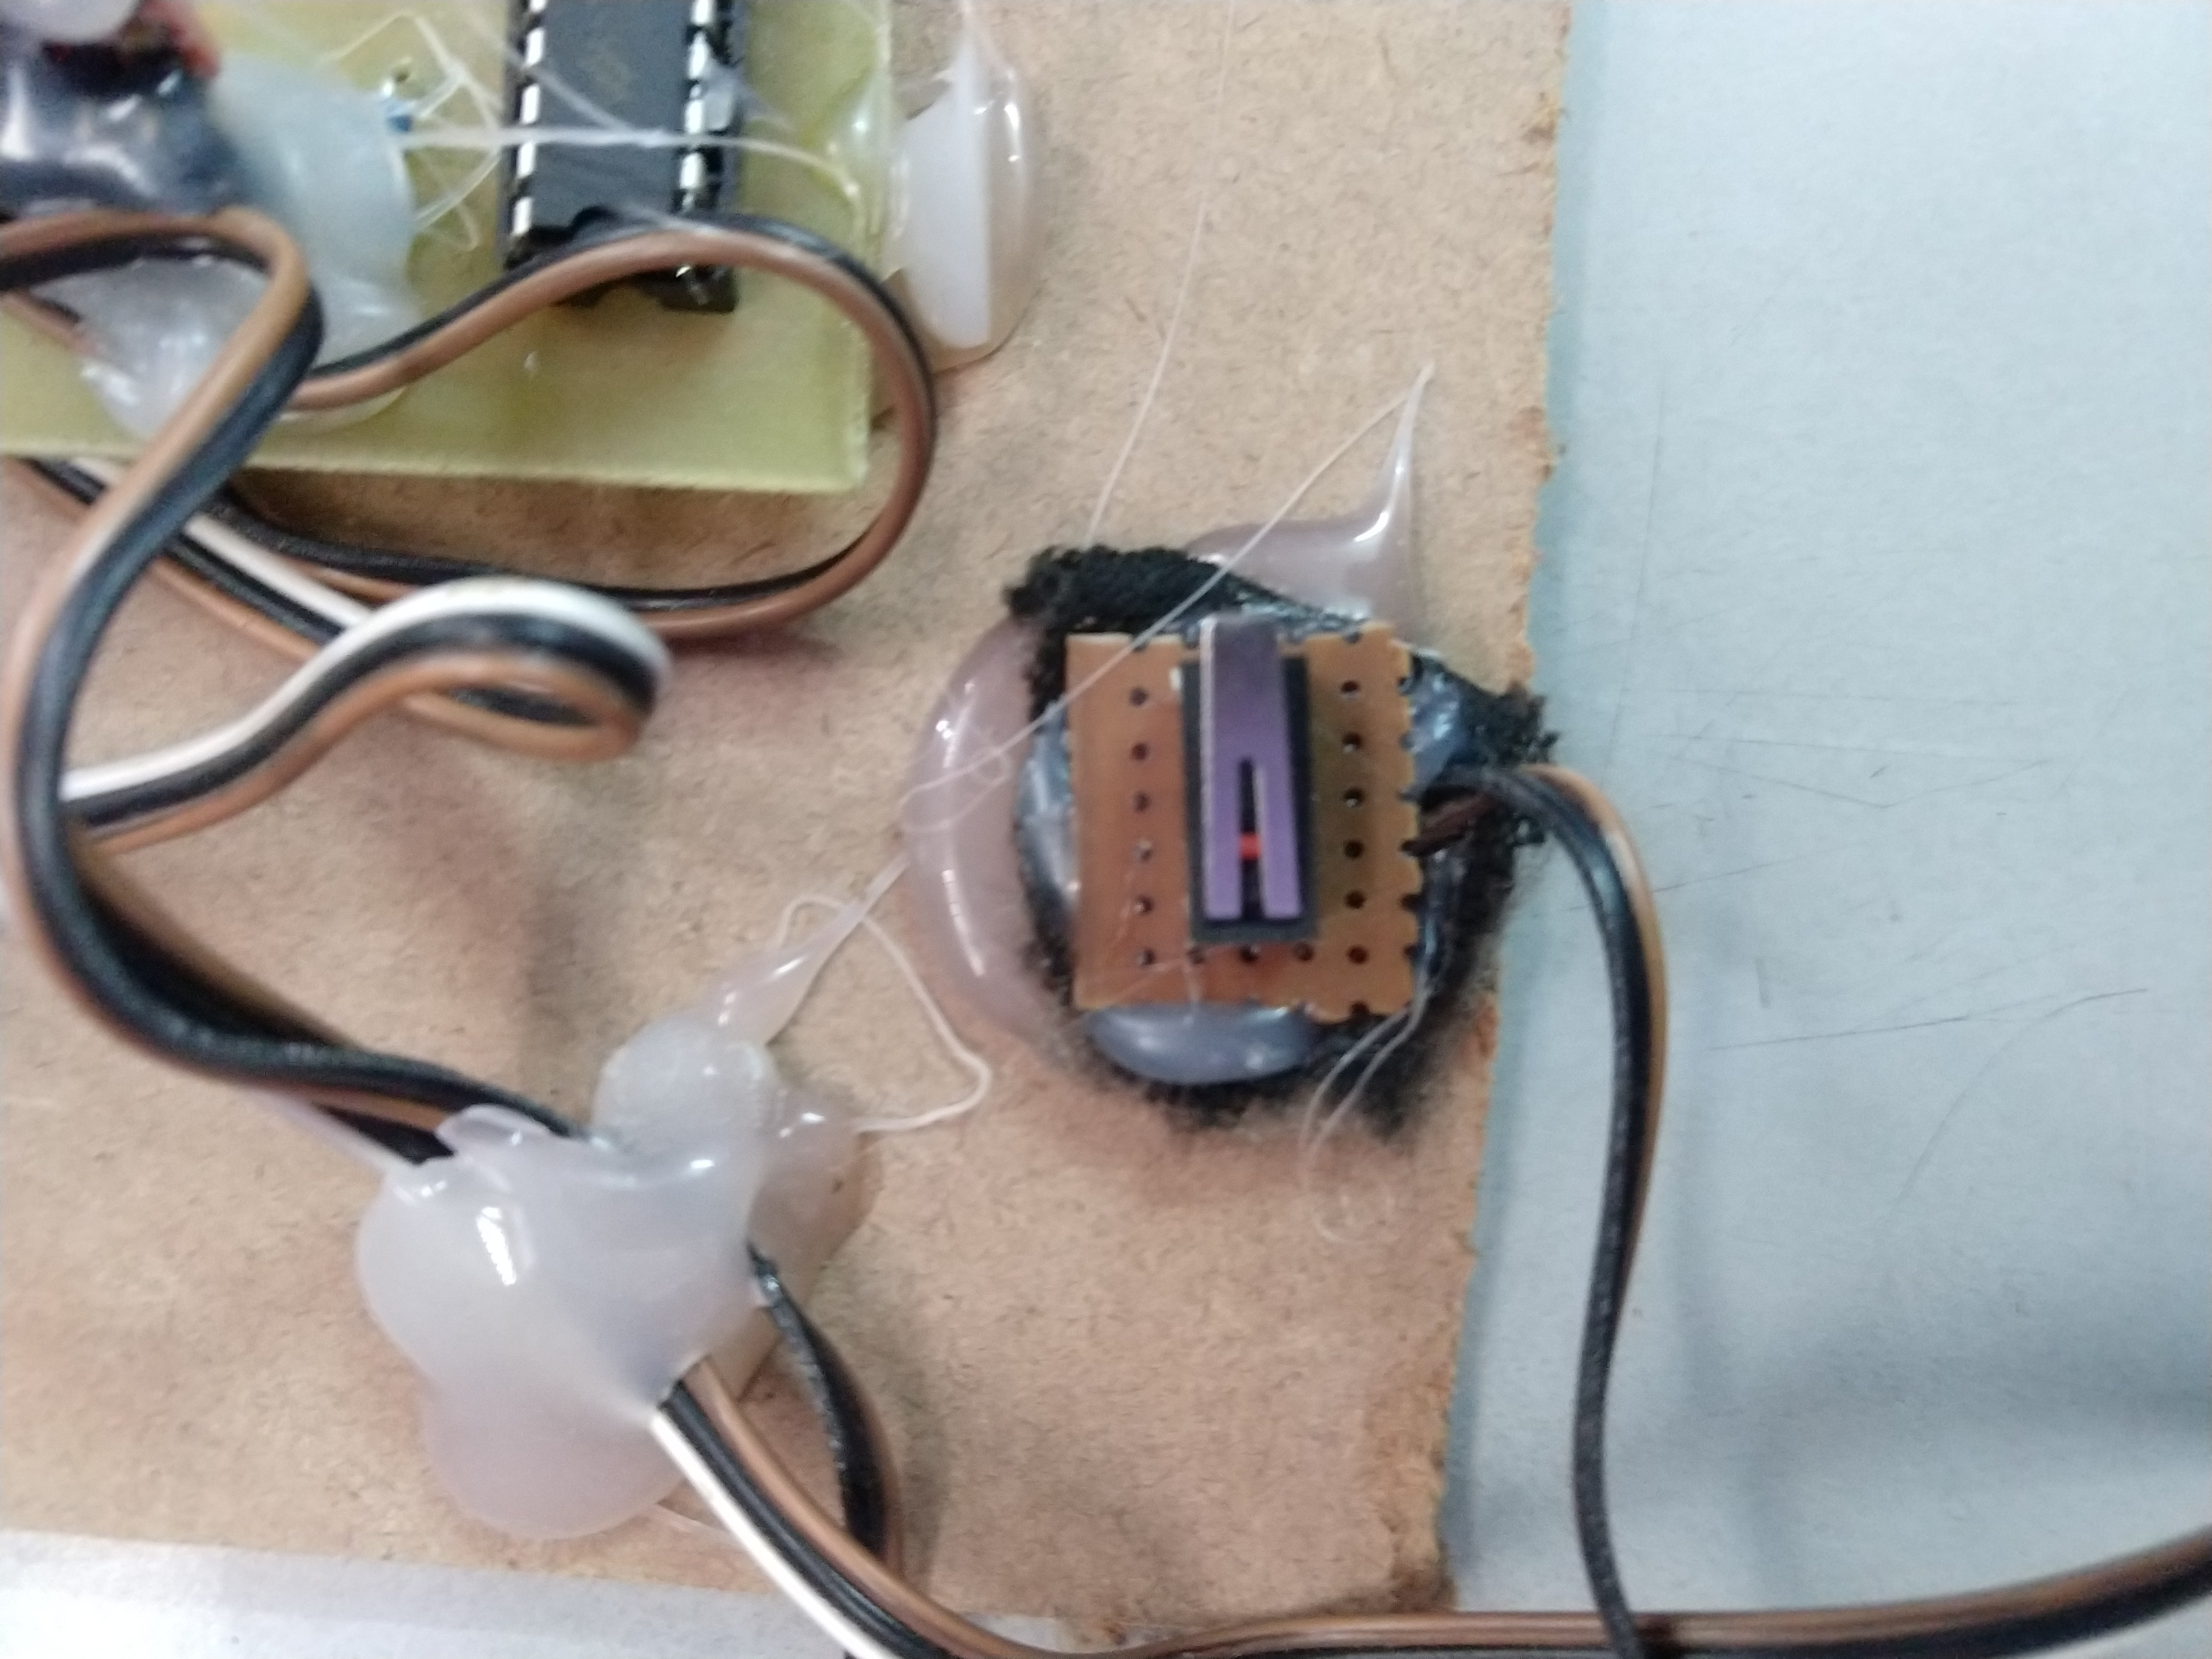
\includegraphics[scale=.08]{IMG_20210617_140428818.jpg}
		\caption{Limit Switch.}
	\end{figure}
	\item Limit switch will be installed at the inner top of the helmet so that the switch will be pressed whenever rider wears the helmet.
	\item Helmet unit will function properly till the limit switch is pressed or we can simply say ON.
	\item Whenever rider remove the helmet limit switch will break the circuit and send signal to HT12E encoder which will transmit data to bike unit via RF receiver.
	\item In bike, signal fro RF receiver will be send to ATmega328 which will send signal to buzzer unit to alarm.
	\item If the rider still doesn't put up the helmet then the ignition will turn OFF
\end{itemize}
\subsection{Rider Got Into An Accident}
\begin{itemize}
	\item For this purpose we have used Reed Switches
	\item When the bike will meet an accident then the glass tube of reed switch will break which will break the entire reed switch section circuit.
	\item When ATmega328 will realise about it then it will send signal to GSM Module to turn ON
	\item GSM Module will send a message that " YOUR BIKE GOT INTO THE ACCIDENT " to the emergency contact which is saved in the code in ATmega328.
	\begin{figure}[h]
		\centering
		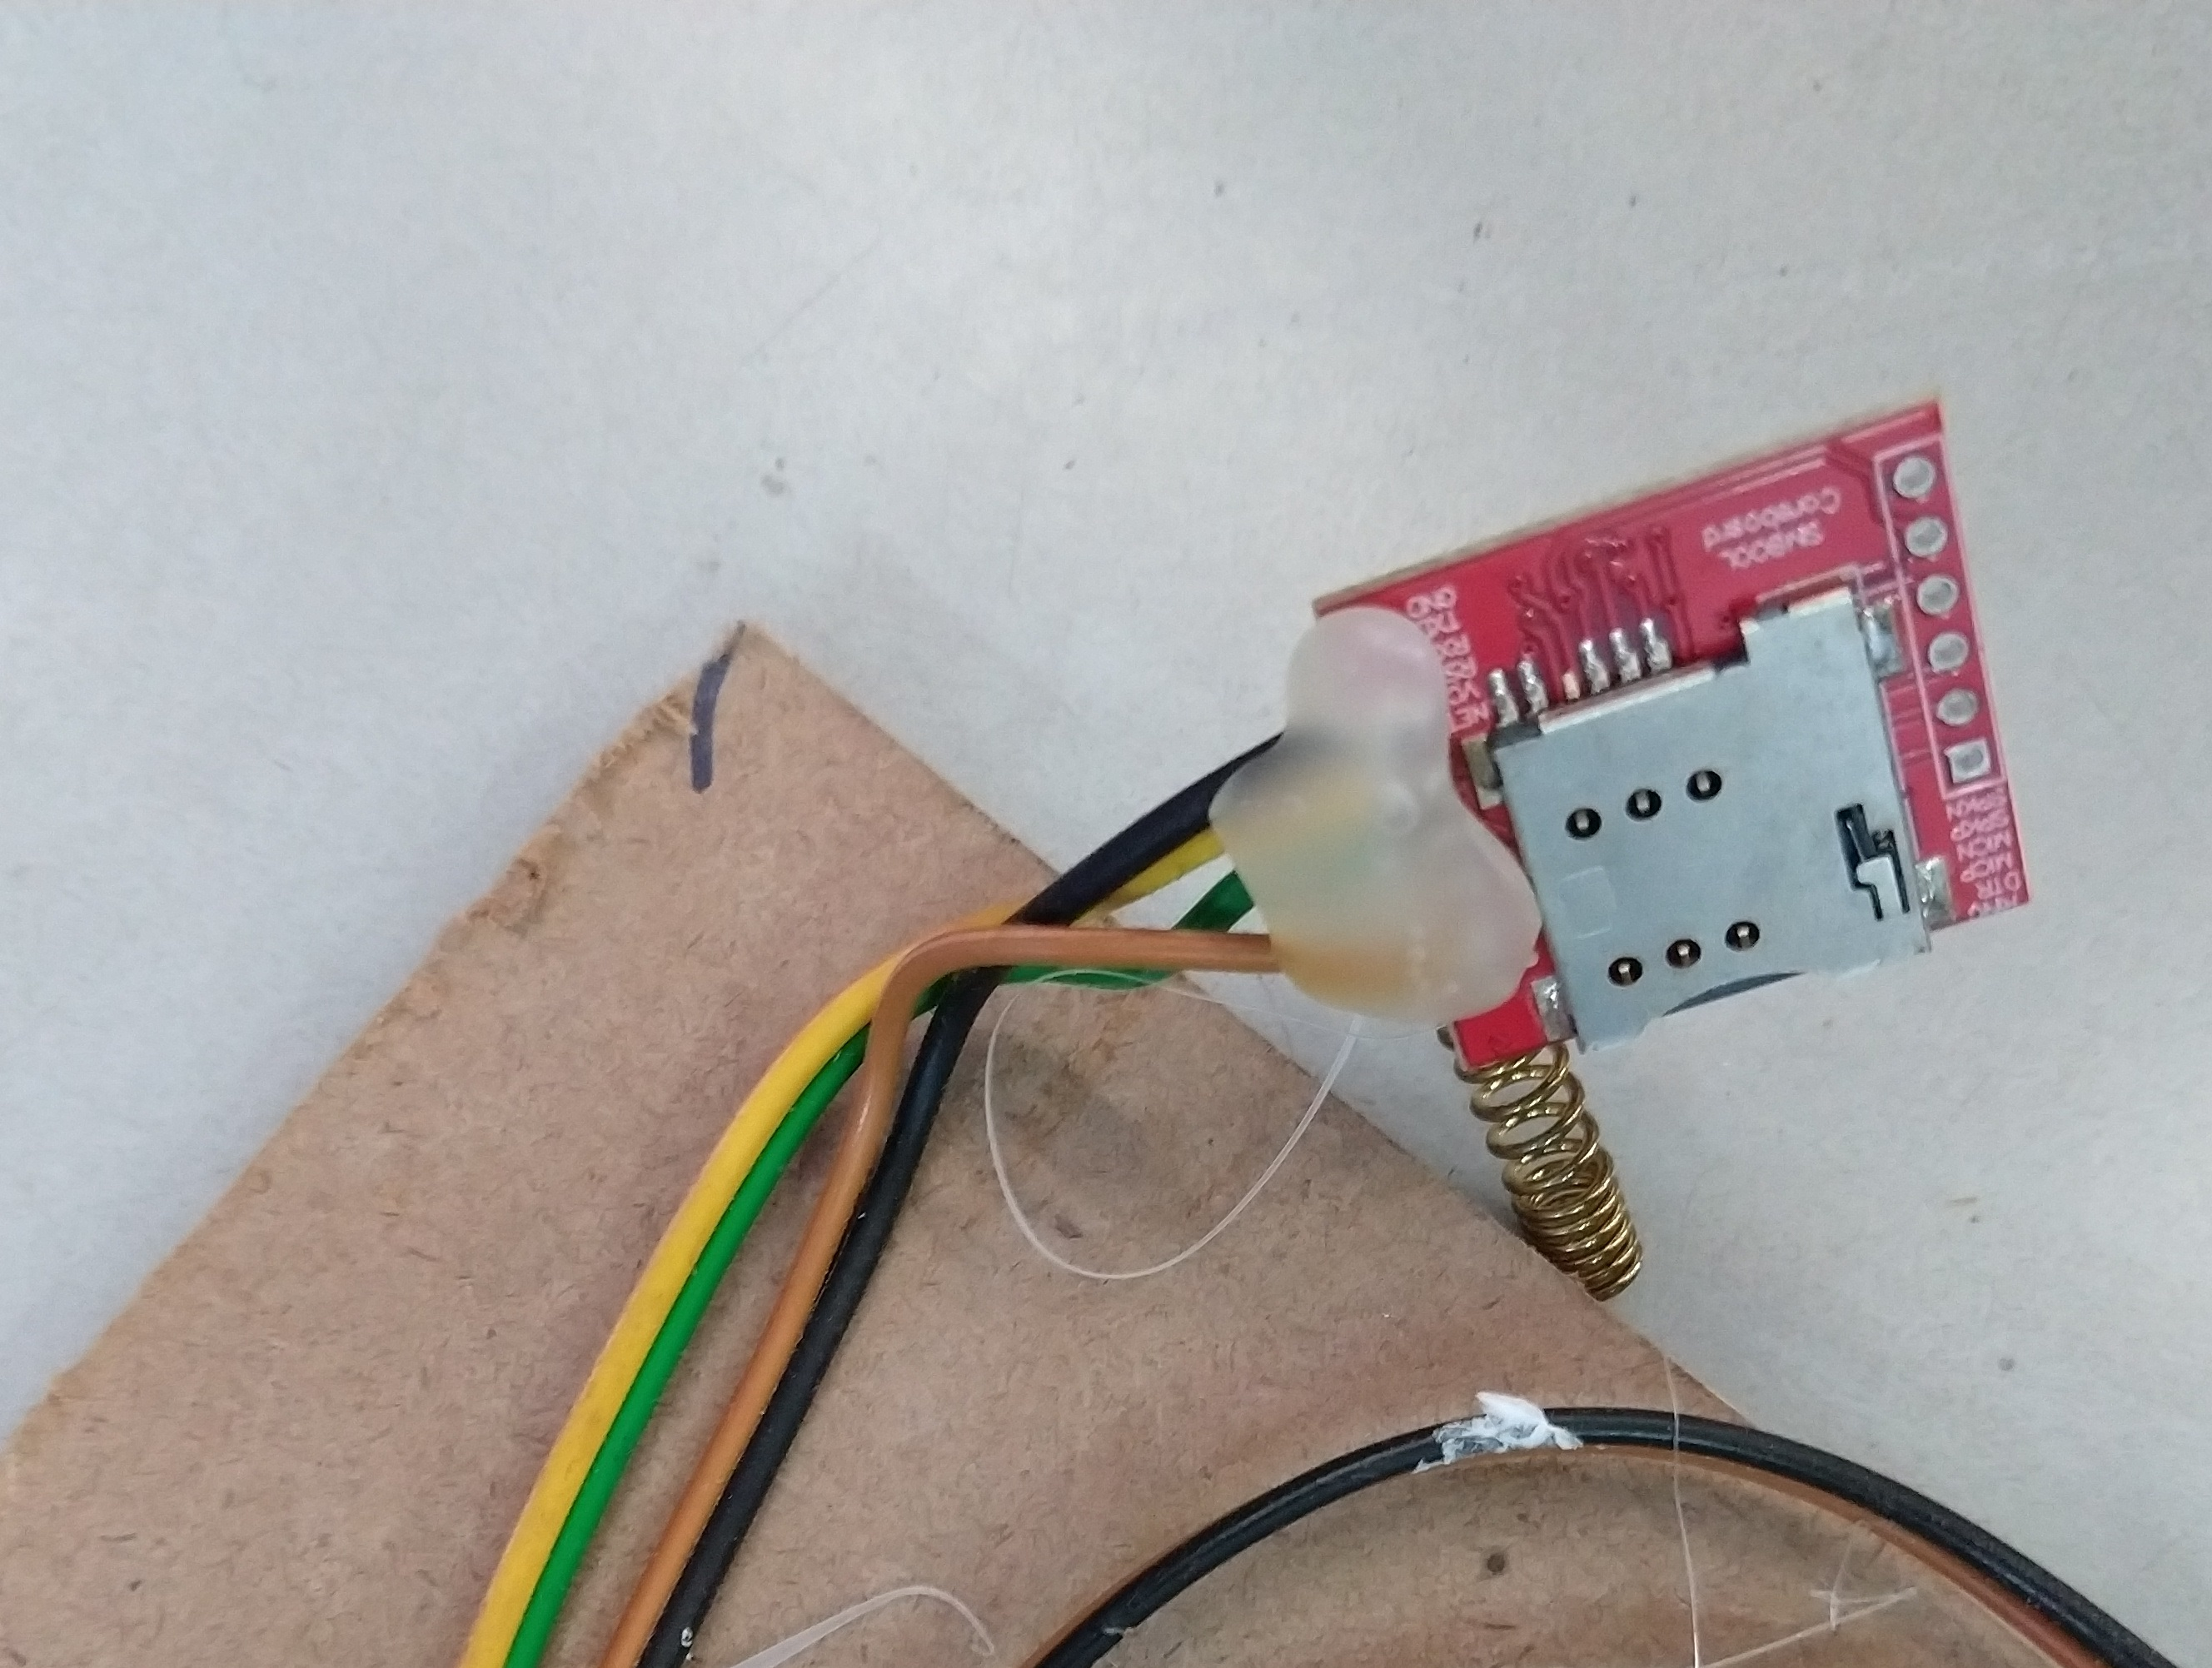
\includegraphics[scale=.06]{IMG_20210617_140334704.jpg}
		\caption{GSM Module.}
	\end{figure}
	\item It will keep sending messages until the reed switch section turn on back or the balance of the sim in GSM Module expires.   
\end{itemize}
